In this thesis we address the 3D single bin-size bin packing problem (3D-SBSBPP). Starting from a set of items of different size the goal is to arrange them in the least ammount of bins of a given fixed size without any overlap between eachother.
In addition to the standard formulation of the problem three additional practical constraints need to be taken into account to satisfy the requests of our use-case:
\begin{itemize}
    \item each item inside a bin should have static stability, meaning that every item should be supported either by the ground or by other items in the same bin
    \item the cage ratio of each used bin should be maximized
    \item each item can be rotated orthogonally along its vertical axis
\end{itemize}

Given a certain placement of items inside a bin of base $W \times D$ with the top of the highest item being at $z_\text{max}$ and the sum of the volume of each item being $V$, the bin's cage ratio is defined as \cref{eq:cage_ratio}.
\begin{equation}
    \label{eq:cage_ratio}
    \text{CR} = \frac{V}{W \cdot D \cdot z_\text{max}}
\end{equation}
A high cage ratio means that even if a bin isn't fully occupied it could potentially be used as a base for other structures, a property which is desirable in some industrial setting.
It is also noted that in a single bin configuration, maximizing cage ratio is equivalent to minimizing $z_\text{max}$. A visual rappresentation of the cage ratio metric is provided in \cref{fig:cage_ratio}.

\begin{figure}[H]
    \scalebox{0.60}{%
    

\tikzset{every picture/.style={line width=0.75pt}} %set default line width to 0.75pt        

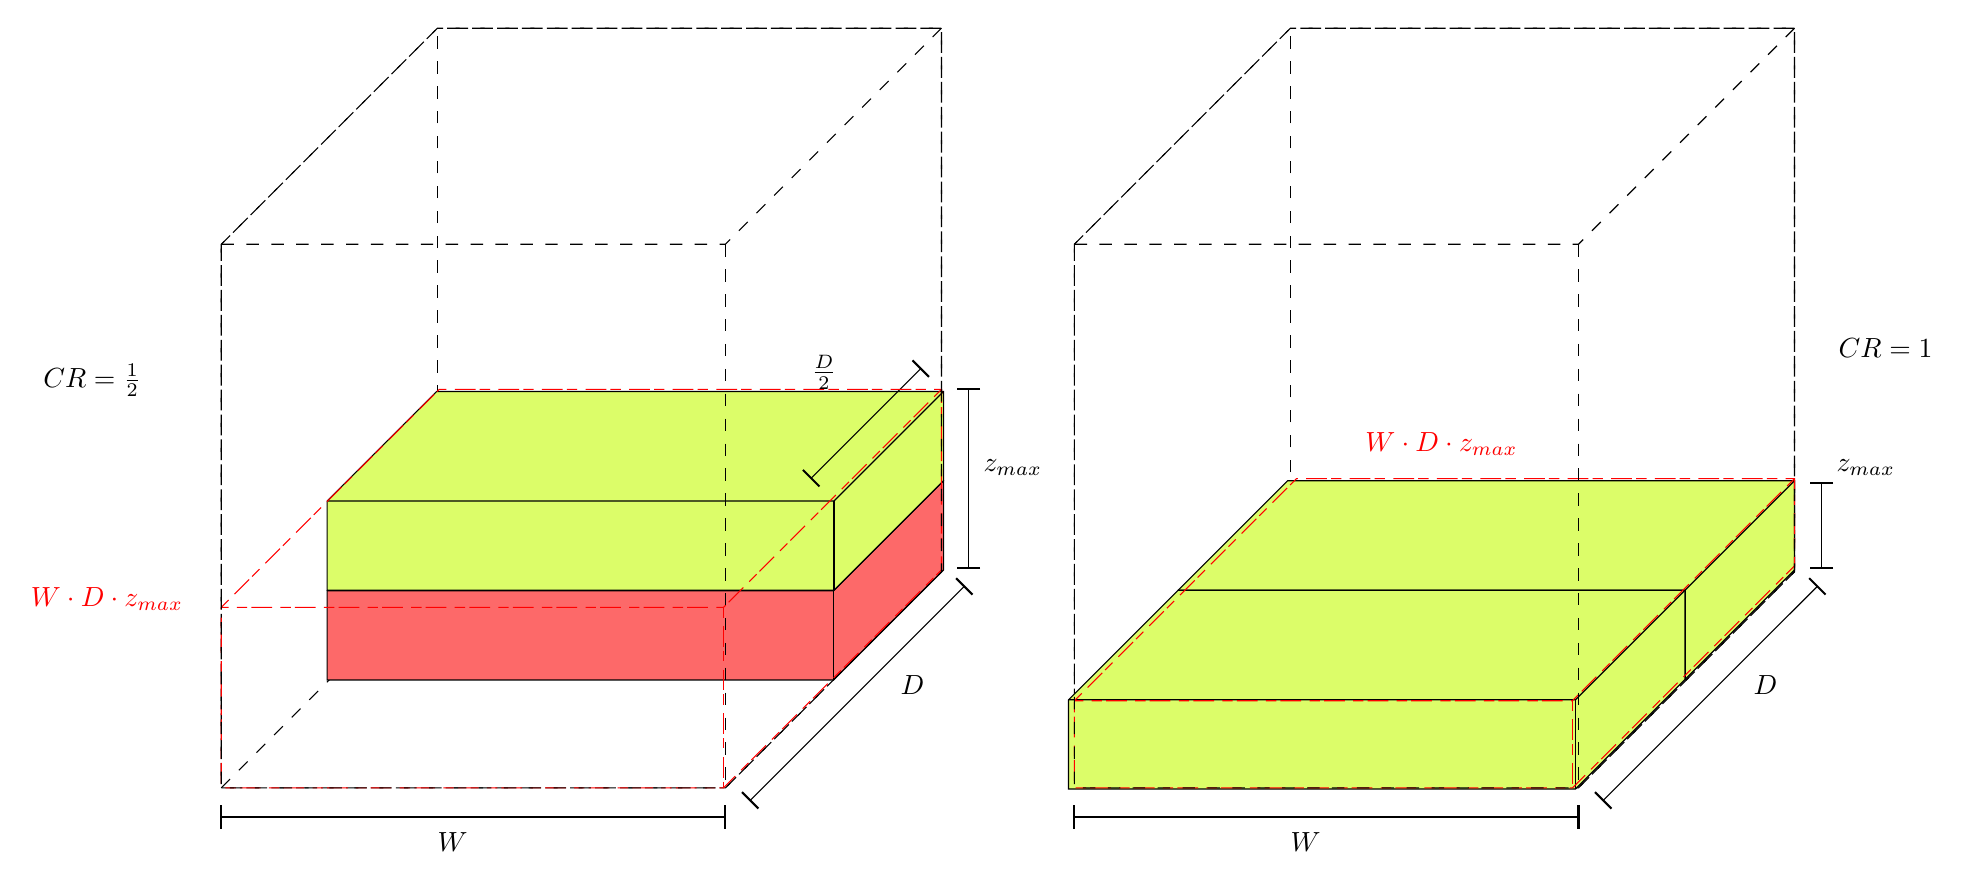
\begin{tikzpicture}[x=0.75pt,y=0.75pt,yscale=-1,xscale=1]
%uncomment if require: \path (0,479); %set diagram left start at 0, and has height of 479

%Shape: Cube [id:dp9446615397697055] 
\draw  [dash pattern={on 4.5pt off 4.5pt}] (917,301.9) -- (812.9,406) -- (570,406) -- (570,144.1) -- (674.1,40) -- (917,40) -- cycle ; \draw  [dash pattern={on 4.5pt off 4.5pt}] (570,406) -- (674.1,301.9) -- (917,301.9) ; \draw  [dash pattern={on 4.5pt off 4.5pt}] (674.1,301.9) -- (674.1,40) ;
%Shape: Cube [id:dp9924623151681093] 
\draw  [fill={rgb, 255:red, 220; green, 253; blue, 105 }  ,fill opacity=1 ] (620,310.78) -- (672.78,258) -- (917,258) -- (917,301) -- (864.22,353.78) -- (620,353.78) -- cycle ; \draw   (917,258) -- (864.22,310.78) -- (620,310.78) ; \draw   (864.22,310.78) -- (864.22,353.78) ;
%Shape: Cube [id:dp4356357707795666] 
\draw  [fill={rgb, 255:red, 220; green, 253; blue, 105 }  ,fill opacity=1 ] (567.22,363.56) -- (620,310.78) -- (864.22,310.78) -- (864.22,353.78) -- (811.44,406.56) -- (567.22,406.56) -- cycle ; \draw   (864.22,310.78) -- (811.44,363.56) -- (567.22,363.56) ; \draw   (811.44,363.56) -- (811.44,406.56) ;
%Shape: Cube [id:dp900981008021689] 
\draw  [dash pattern={on 4.5pt off 4.5pt}] (506,301.9) -- (401.9,406) -- (159,406) -- (159,144.1) -- (263.1,40) -- (506,40) -- cycle ; \draw  [dash pattern={on 4.5pt off 4.5pt}] (159,406) -- (263.1,301.9) -- (506,301.9) ; \draw  [dash pattern={on 4.5pt off 4.5pt}] (263.1,301.9) -- (263.1,40) ;
%Shape: Cube [id:dp9462720863667783] 
\draw  [fill={rgb, 255:red, 253; green, 105; blue, 105 }  ,fill opacity=1 ] (210,311) -- (263,258) -- (507,258) -- (507,301) -- (454,354) -- (210,354) -- cycle ; \draw   (507,258) -- (454,311) -- (210,311) ; \draw   (454,311) -- (454,354) ;
%Shape: Cube [id:dp20686523528460465] 
\draw  [fill={rgb, 255:red, 220; green, 253; blue, 105 }  ,fill opacity=1 ] (210,267.78) -- (262.78,215) -- (507,215) -- (507,258) -- (454.22,310.78) -- (210,310.78) -- cycle ; \draw   (507,215) -- (454.22,267.78) -- (210,267.78) ; \draw   (454.22,267.78) -- (454.22,310.78) ;
%Straight Lines [id:da9583369995131138] 
\draw    (496,204) -- (443.22,256.78) ;
\draw [shift={(443.22,256.78)}, rotate = 315] [color={rgb, 255:red, 0; green, 0; blue, 0 }  ][line width=0.75]    (0,5.59) -- (0,-5.59)   ;
\draw [shift={(496,204)}, rotate = 315] [color={rgb, 255:red, 0; green, 0; blue, 0 }  ][line width=0.75]    (0,5.59) -- (0,-5.59)   ;
%Straight Lines [id:da4480701288134522] 
\draw    (401.9,420) -- (159,420) ;
\draw [shift={(159,420)}, rotate = 360] [color={rgb, 255:red, 0; green, 0; blue, 0 }  ][line width=0.75]    (0,5.59) -- (0,-5.59)   ;
\draw [shift={(401.9,420)}, rotate = 360] [color={rgb, 255:red, 0; green, 0; blue, 0 }  ][line width=0.75]    (0,5.59) -- (0,-5.59)   ;
%Straight Lines [id:da9761873387202039] 
\draw    (517,308.9) -- (413.86,412) ;
\draw [shift={(413.86,412)}, rotate = 315.01] [color={rgb, 255:red, 0; green, 0; blue, 0 }  ][line width=0.75]    (0,5.59) -- (0,-5.59)   ;
\draw [shift={(517,308.9)}, rotate = 315.01] [color={rgb, 255:red, 0; green, 0; blue, 0 }  ][line width=0.75]    (0,5.59) -- (0,-5.59)   ;
%Straight Lines [id:da1211437330301477] 
\draw    (519,214) -- (519,299.86) ;
\draw [shift={(519,299.86)}, rotate = 270] [color={rgb, 255:red, 0; green, 0; blue, 0 }  ][line width=0.75]    (0,5.59) -- (0,-5.59)   ;
\draw [shift={(519,214)}, rotate = 270] [color={rgb, 255:red, 0; green, 0; blue, 0 }  ][line width=0.75]    (0,5.59) -- (0,-5.59)   ;
%Shape: Cube [id:dp6016430781165488] 
\draw  [color={rgb, 255:red, 255; green, 0; blue, 0 }  ,draw opacity=1 ][dash pattern={on 3.75pt off 3pt on 7.5pt off 1.5pt}] (159,319) -- (264,214) -- (506,214) -- (506,301) -- (401,406) -- (159,406) -- cycle ; \draw  [color={rgb, 255:red, 255; green, 0; blue, 0 }  ,draw opacity=1 ][dash pattern={on 3.75pt off 3pt on 7.5pt off 1.5pt}] (506,214) -- (401,319) -- (159,319) ; \draw  [color={rgb, 255:red, 255; green, 0; blue, 0 }  ,draw opacity=1 ][dash pattern={on 3.75pt off 3pt on 7.5pt off 1.5pt}] (401,319) -- (401,406) ;
%Shape: Cube [id:dp9858212525551202] 
\draw  [dash pattern={on 4.5pt off 4.5pt}] (159,144.1) -- (263.1,40) -- (506,40) -- (506,301.9) -- (401.9,406) -- (159,406) -- cycle ; \draw  [dash pattern={on 4.5pt off 4.5pt}] (506,40) -- (401.9,144.1) -- (159,144.1) ; \draw  [dash pattern={on 4.5pt off 4.5pt}] (401.9,144.1) -- (401.9,406) ;
%Straight Lines [id:da4537070040642701] 
\draw    (812.9,420) -- (570,420) ;
\draw [shift={(570,420)}, rotate = 360] [color={rgb, 255:red, 0; green, 0; blue, 0 }  ][line width=0.75]    (0,5.59) -- (0,-5.59)   ;
\draw [shift={(812.9,420)}, rotate = 360] [color={rgb, 255:red, 0; green, 0; blue, 0 }  ][line width=0.75]    (0,5.59) -- (0,-5.59)   ;
%Straight Lines [id:da13051427322471099] 
\draw    (928,308.9) -- (824.86,412) ;
\draw [shift={(824.86,412)}, rotate = 315.01] [color={rgb, 255:red, 0; green, 0; blue, 0 }  ][line width=0.75]    (0,5.59) -- (0,-5.59)   ;
\draw [shift={(928,308.9)}, rotate = 315.01] [color={rgb, 255:red, 0; green, 0; blue, 0 }  ][line width=0.75]    (0,5.59) -- (0,-5.59)   ;
%Straight Lines [id:da38828166025774113] 
\draw    (930,259) -- (930,299.86) ;
\draw [shift={(930,299.86)}, rotate = 270] [color={rgb, 255:red, 0; green, 0; blue, 0 }  ][line width=0.75]    (0,5.59) -- (0,-5.59)   ;
\draw [shift={(930,259)}, rotate = 270] [color={rgb, 255:red, 0; green, 0; blue, 0 }  ][line width=0.75]    (0,5.59) -- (0,-5.59)   ;
%Shape: Cube [id:dp33203292048167843] 
\draw  [color={rgb, 255:red, 255; green, 0; blue, 0 }  ,draw opacity=1 ][dash pattern={on 3.75pt off 3pt on 7.5pt off 1.5pt}] (570,364) -- (677,257) -- (917,257) -- (917,299) -- (810,406) -- (570,406) -- cycle ; \draw  [color={rgb, 255:red, 255; green, 0; blue, 0 }  ,draw opacity=1 ][dash pattern={on 3.75pt off 3pt on 7.5pt off 1.5pt}] (917,257) -- (810,364) -- (570,364) ; \draw  [color={rgb, 255:red, 255; green, 0; blue, 0 }  ,draw opacity=1 ][dash pattern={on 3.75pt off 3pt on 7.5pt off 1.5pt}] (810,364) -- (810,406) ;
%Shape: Cube [id:dp6959350788468752] 
\draw  [dash pattern={on 4.5pt off 4.5pt}] (570,144.1) -- (674.1,40) -- (917,40) -- (917,301.9) -- (812.9,406) -- (570,406) -- cycle ; \draw  [dash pattern={on 4.5pt off 4.5pt}] (917,40) -- (812.9,144.1) -- (570,144.1) ; \draw  [dash pattern={on 4.5pt off 4.5pt}] (812.9,144.1) -- (812.9,406) ;

% Text Node
\draw (442,196.4) node [anchor=north west][inner sep=0.75pt]    {$\frac{D}{2}$};
% Text Node
\draw (262,426.4) node [anchor=north west][inner sep=0.75pt]    {$W$};
% Text Node
\draw (485,350.4) node [anchor=north west][inner sep=0.75pt]    {$D$};
% Text Node
\draw (72,200.4) node [anchor=north west][inner sep=0.75pt]    {$CR=\frac{1}{2}$};
% Text Node
\draw (525,246.4) node [anchor=north west][inner sep=0.75pt]    {$z_{\text{max}}$};
% Text Node
\draw (66,308.4) node [anchor=north west][inner sep=0.75pt]  [color={rgb, 255:red, 255; green, 0; blue, 0 }  ,opacity=1 ]  {$W\cdot D\cdot z_{\text{max}}$};
% Text Node
\draw (673,426.4) node [anchor=north west][inner sep=0.75pt]    {$W$};
% Text Node
\draw (896,350.4) node [anchor=north west][inner sep=0.75pt]    {$D$};
% Text Node
\draw (937,188.4) node [anchor=north west][inner sep=0.75pt]    {$CR=1$};
% Text Node
\draw (936,246.4) node [anchor=north west][inner sep=0.75pt]    {$z_{\text{max}}$};
% Text Node
\draw (709,233.4) node [anchor=north west][inner sep=0.75pt]  [color={rgb, 255:red, 255; green, 0; blue, 0 }  ,opacity=1 ]  {$W\cdot D\cdot z_{\text{max}}$};


\end{tikzpicture}

    }
    \caption{Cage ratio of two different bin configurations}
    \label{fig:cage_ratio}
\end{figure}

Our notion of vertical support stems from rules imposed by the industry and from the literature on Pallet Loading Problems and Container Loading Problems where stability is usually ensured between horizontal or vertical slices of items as a constraint on the minimum ammount of area which rests on other items (as for ex. \citep{elhedhli2019three,kurpel2020exact,paquay2016mixed}).
Given a support area threshold which is usually equal to $\alpha_s=0.7$ and a tollerance which in our case is equal to $\beta_s=1\text{cm}$, we can define an item as supported if
\begin{enumerate}
    \item the sum of overlap area with every other item on which it is resting is greater then $\alpha_s$ times it's area \label{support:area_support}
    \item the number of its corners resting on another item is greater than 3 and condition \ref{support:area_support} holds with a lower threshold $\alpha^\prime_s < \alpha_s$ \label{support:vertex_support}
\end{enumerate}
A visual rappresentation of the condition of support is illustrated in \cref{fig:support}.

\begin{figure}[H]
    \scalebox{0.55}{%
    

\tikzset{every picture/.style={line width=0.75pt}} %set default line width to 0.75pt        

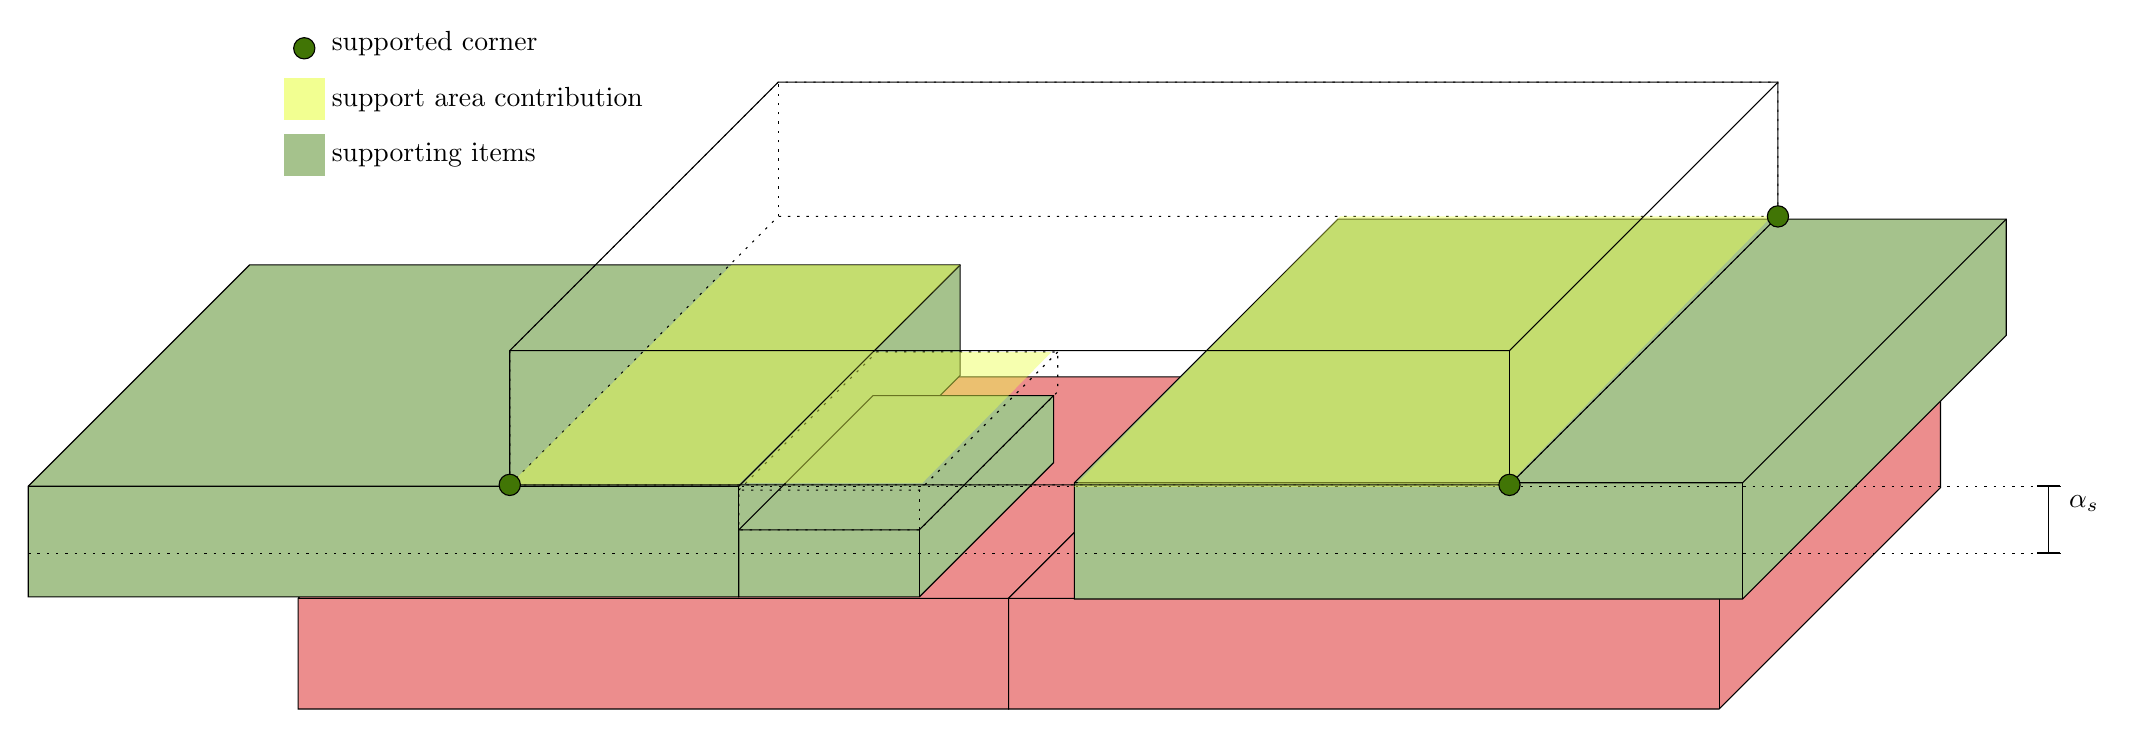
\begin{tikzpicture}[x=0.75pt,y=0.75pt,yscale=-1,xscale=1]
%uncomment if require: \path (0,479); %set diagram left start at 0, and has height of 479

%Shape: Cube [id:dp9411979483763162] 
\draw  [fill={rgb, 255:red, 236; green, 141; blue, 141 }  ,fill opacity=1 ] (194,306.67) -- (300.67,200) -- (643,200) -- (643,253.33) -- (536.33,360) -- (194,360) -- cycle ; \draw   (643,200) -- (536.33,306.67) -- (194,306.67) ; \draw   (536.33,306.67) -- (536.33,360) ;
%Shape: Cube [id:dp993645103603593] 
\draw  [fill={rgb, 255:red, 236; green, 141; blue, 141 }  ,fill opacity=1 ] (536.33,306.67) -- (643,200) -- (985.33,200) -- (985.33,253.33) -- (878.67,360) -- (536.33,360) -- cycle ; \draw   (985.33,200) -- (878.67,306.67) -- (536.33,306.67) ; \draw   (878.67,306.67) -- (878.67,360) ;
%Shape: Cube [id:dp23986673546182513] 
\draw  [fill={rgb, 255:red, 165; green, 194; blue, 140 }  ,fill opacity=1 ] (64,252.67) -- (170.67,146) -- (513,146) -- (513,199.33) -- (406.33,306) -- (64,306) -- cycle ; \draw   (513,146) -- (406.33,252.67) -- (64,252.67) ; \draw   (406.33,252.67) -- (406.33,306) ;
%Shape: Cube [id:dp5474008601617114] 
\draw  [fill={rgb, 255:red, 165; green, 194; blue, 140 }  ,fill opacity=1 ] (406.33,273.67) -- (471,209) -- (558,209) -- (558,241.33) -- (493.33,306) -- (406.33,306) -- cycle ; \draw   (558,209) -- (493.33,273.67) -- (406.33,273.67) ; \draw   (493.33,273.67) -- (493.33,306) ;
%Shape: Cube [id:dp7313777533771082] 
\draw  [fill={rgb, 255:red, 165; green, 194; blue, 140 }  ,fill opacity=1 ] (568,251) -- (695,124) -- (1017,124) -- (1017,180) -- (890,307) -- (568,307) -- cycle ; \draw   (1017,124) -- (890,251) -- (568,251) ; \draw   (890,251) -- (890,307) ;
%Shape: Cube [id:dp9978562503762016] 
\draw  [dash pattern={on 0.84pt off 2.51pt}] (907,122.67) -- (777.67,252) -- (296,252) -- (296,187.33) -- (425.33,58) -- (907,58) -- cycle ; \draw  [dash pattern={on 0.84pt off 2.51pt}] (296,252) -- (425.33,122.67) -- (907,122.67) ; \draw  [dash pattern={on 0.84pt off 2.51pt}] (425.33,122.67) -- (425.33,58) ;
%Shape: Cube [id:dp48964002783685845] 
\draw  [color={rgb, 255:red, 0; green, 0; blue, 0 }  ,draw opacity=1 ][fill={rgb, 255:red, 255; green, 255; blue, 255 }  ,fill opacity=0 ][dash pattern={on 0.84pt off 2.51pt}] (406.33,254.53) -- (472.86,188) -- (560,188) -- (560,207.14) -- (493.47,273.67) -- (406.33,273.67) -- cycle ; \draw  [color={rgb, 255:red, 0; green, 0; blue, 0 }  ,draw opacity=1 ][dash pattern={on 0.84pt off 2.51pt}] (560,188) -- (493.47,254.53) -- (406.33,254.53) ; \draw  [color={rgb, 255:red, 0; green, 0; blue, 0 }  ,draw opacity=1 ][dash pattern={on 0.84pt off 2.51pt}] (493.47,254.53) -- (493.47,273.67) ;
%Straight Lines [id:da26590658600836115] 
\draw    (1037.33,252.67) -- (1037.33,285) ;
\draw [shift={(1037.33,285)}, rotate = 270] [color={rgb, 255:red, 0; green, 0; blue, 0 }  ][line width=0.75]    (0,5.59) -- (0,-5.59)   ;
\draw [shift={(1037.33,252.67)}, rotate = 270] [color={rgb, 255:red, 0; green, 0; blue, 0 }  ][line width=0.75]    (0,5.59) -- (0,-5.59)   ;
%Straight Lines [id:da8302030012021052] 
\draw  [dash pattern={on 0.84pt off 2.51pt}]  (64,285) -- (1044,285) ;
%Straight Lines [id:da5354149137938202] 
\draw  [dash pattern={on 0.84pt off 2.51pt}]  (64,252.67) -- (1044,252.67) ;
%Shape: Parallelogram [id:dp4597753988697182] 
\draw  [color={rgb, 255:red, 0; green, 0; blue, 0 }  ,draw opacity=0 ][fill={rgb, 255:red, 234; green, 255; blue, 77 }  ,fill opacity=0.45 ] (403,146) -- (513,146) -- (406,252) -- (296,252) -- cycle ;
%Shape: Parallelogram [id:dp9407100355043312] 
\draw  [color={rgb, 255:red, 0; green, 0; blue, 0 }  ,draw opacity=0 ][fill={rgb, 255:red, 234; green, 255; blue, 77 }  ,fill opacity=0.45 ] (471,188) -- (557,188) -- (494.86,251) -- (408.86,251) -- cycle ;
%Shape: Parallelogram [id:dp5499917231467685] 
\draw  [color={rgb, 255:red, 0; green, 0; blue, 0 }  ,draw opacity=0 ][fill={rgb, 255:red, 234; green, 255; blue, 77 }  ,fill opacity=0.45 ] (696,122.67) -- (904,122.67) -- (775.67,253) -- (567.67,253) -- cycle ;
%Shape: Cube [id:dp21506487392572304] 
\draw   (296,187.33) -- (425.33,58) -- (907,58) -- (907,122.67) -- (777.67,252) -- (296,252) -- cycle ; \draw   (907,58) -- (777.67,187.33) -- (296,187.33) ; \draw   (777.67,187.33) -- (777.67,252) ;
%Shape: Rectangle [id:dp8515603217170198] 
\draw  [color={rgb, 255:red, 0; green, 0; blue, 0 }  ,draw opacity=0 ][fill={rgb, 255:red, 234; green, 255; blue, 77 }  ,fill opacity=0.62 ] (187,56) -- (207,56) -- (207,76) -- (187,76) -- cycle ;
%Shape: Rectangle [id:dp8969674268045522] 
\draw  [color={rgb, 255:red, 0; green, 0; blue, 0 }  ,draw opacity=0 ][fill={rgb, 255:red, 165; green, 194; blue, 140 }  ,fill opacity=1 ] (187,83) -- (207,83) -- (207,103) -- (187,103) -- cycle ;
%Shape: Circle [id:dp08410160878408413] 
\draw  [fill={rgb, 255:red, 65; green, 117; blue, 5 }  ,fill opacity=1 ] (290.88,252) .. controls (290.88,249.17) and (293.17,246.88) .. (296,246.88) .. controls (298.83,246.88) and (301.13,249.17) .. (301.13,252) .. controls (301.13,254.83) and (298.83,257.13) .. (296,257.13) .. controls (293.17,257.13) and (290.88,254.83) .. (290.88,252) -- cycle ;
%Shape: Circle [id:dp20799682119759832] 
\draw  [fill={rgb, 255:red, 65; green, 117; blue, 5 }  ,fill opacity=1 ] (772.54,252) .. controls (772.54,249.17) and (774.84,246.88) .. (777.67,246.88) .. controls (780.5,246.88) and (782.79,249.17) .. (782.79,252) .. controls (782.79,254.83) and (780.5,257.13) .. (777.67,257.13) .. controls (774.84,257.13) and (772.54,254.83) .. (772.54,252) -- cycle ;
%Shape: Circle [id:dp9242580914559287] 
\draw  [fill={rgb, 255:red, 65; green, 117; blue, 5 }  ,fill opacity=1 ] (901.88,122.67) .. controls (901.88,119.84) and (904.17,117.54) .. (907,117.54) .. controls (909.83,117.54) and (912.13,119.84) .. (912.13,122.67) .. controls (912.13,125.5) and (909.83,127.79) .. (907,127.79) .. controls (904.17,127.79) and (901.88,125.5) .. (901.88,122.67) -- cycle ;
%Shape: Circle [id:dp40386474009325335] 
\draw  [fill={rgb, 255:red, 65; green, 117; blue, 5 }  ,fill opacity=1 ] (191.88,41.67) .. controls (191.88,38.84) and (194.17,36.54) .. (197,36.54) .. controls (199.83,36.54) and (202.13,38.84) .. (202.13,41.67) .. controls (202.13,44.5) and (199.83,46.79) .. (197,46.79) .. controls (194.17,46.79) and (191.88,44.5) .. (191.88,41.67) -- cycle ;

% Text Node
\draw (1046,256.07) node [anchor=north west][inner sep=0.75pt]    {$\alpha _{s}$};
% Text Node
\draw (209,59) node [anchor=north west][inner sep=0.75pt]   [align=left] {support area contribution};
% Text Node
\draw (209,86) node [anchor=north west][inner sep=0.75pt]   [align=left] {supporting items};
% Text Node
\draw (209,32) node [anchor=north west][inner sep=0.75pt]   [align=left] {supported corner};


\end{tikzpicture}

    }
    \caption{Rappresentation of an item with vertical support given $\alpha_s = 0.5, \beta_s$}
    \label{fig:support}
\end{figure}

\newpage
Given the definitions of our practical constraints, a conceptual formulation of our model would be
\begin{eqnarray*}
    \textbf{minimize} & \text{number of used bins} \\
                        & \text{unused volume of each bin under $z_\text{max}$} \\
    \textbf{subject to} & \text{all items assigned to one and only one bin} \\
                                      & \text{all items within the bin dimensions} \\
                                      & \text{no overlaps between items in the same bin} \\
                                      & \text{all items with vertical support} \\
\end{eqnarray*}

In \cref{sec:milp} a mixed integer linear programming model for the 3D-SBSBPP is presented and it's later extended to include orthogonal rotations in \cref{subsec:orthogonal_rotations} and vertical support constraints limited to condition \ref{support:area_support} (area support) in \cref{subsec:vertical_support_formulation}.
Cage ratio isn't directly included in the proposed MILP formulation since the evaluation of the heuristic with the model was done in a single bin configuration where minimizing the maximum height of the bin is equivalent to minimizing the cage ratio.

\section{3D single bin-size bin packing problem}
\label{sec:milp}%
Let $I = \{1,\dots, n \}$ be the set of items that needs to be packed, $B = \{1,\dots, m \}$ the set of bins to evaluate of fixed dimensions $W \times D \times H$.
Each item $i \in I$ is characterized by a given width, depth  and height $(w_i, d_i, h_i)$. 
Let us introduce three continuous variables that identify the position of the bottom front left corner of an item $(x_i, y_i, h_i)$ as seen in \cref{fig:coordinate_system}.
We can now introduce a set of integer variables $v_{b}$ which will be 1 if bin $b \in B$ will be used in the solution and 0 otherwhise. A set of integer variable $u_{ib}$ which will be 1 if item $i \in I$ will be placed in bin $b \in B$ and 0 otherwhise.
In order to check for overlaps three sets of integer variables are introduced for each axis of possible overlap that are used to determine if there is a clear order of precedence on at least on axis. This formulation is also usually used in scheduling problems.
The three sets of variables are $x^p_{ij}$ which will take the value of one if item $i \in I$ precedes item $j \in I$ over axis $x$ given that item $i$ precedes item $j$ if $x_i + w_i \le x_j$ and 0 otherwhise. 
The other two sets are defined in a similar way over the remaining axis $y^p_{ij}$ and $z^p_{ij}$. An additional set of continuous variables $z_b^\text{max}$ is introduced which will assume the value of the maximum $x_i + h_i$ of the items $i \in I$ placed in bin $b \in B$.

\begin{figure}
    \scalebox{0.62}{%
    

\tikzset{every picture/.style={line width=0.75pt}} %set default line width to 0.75pt        

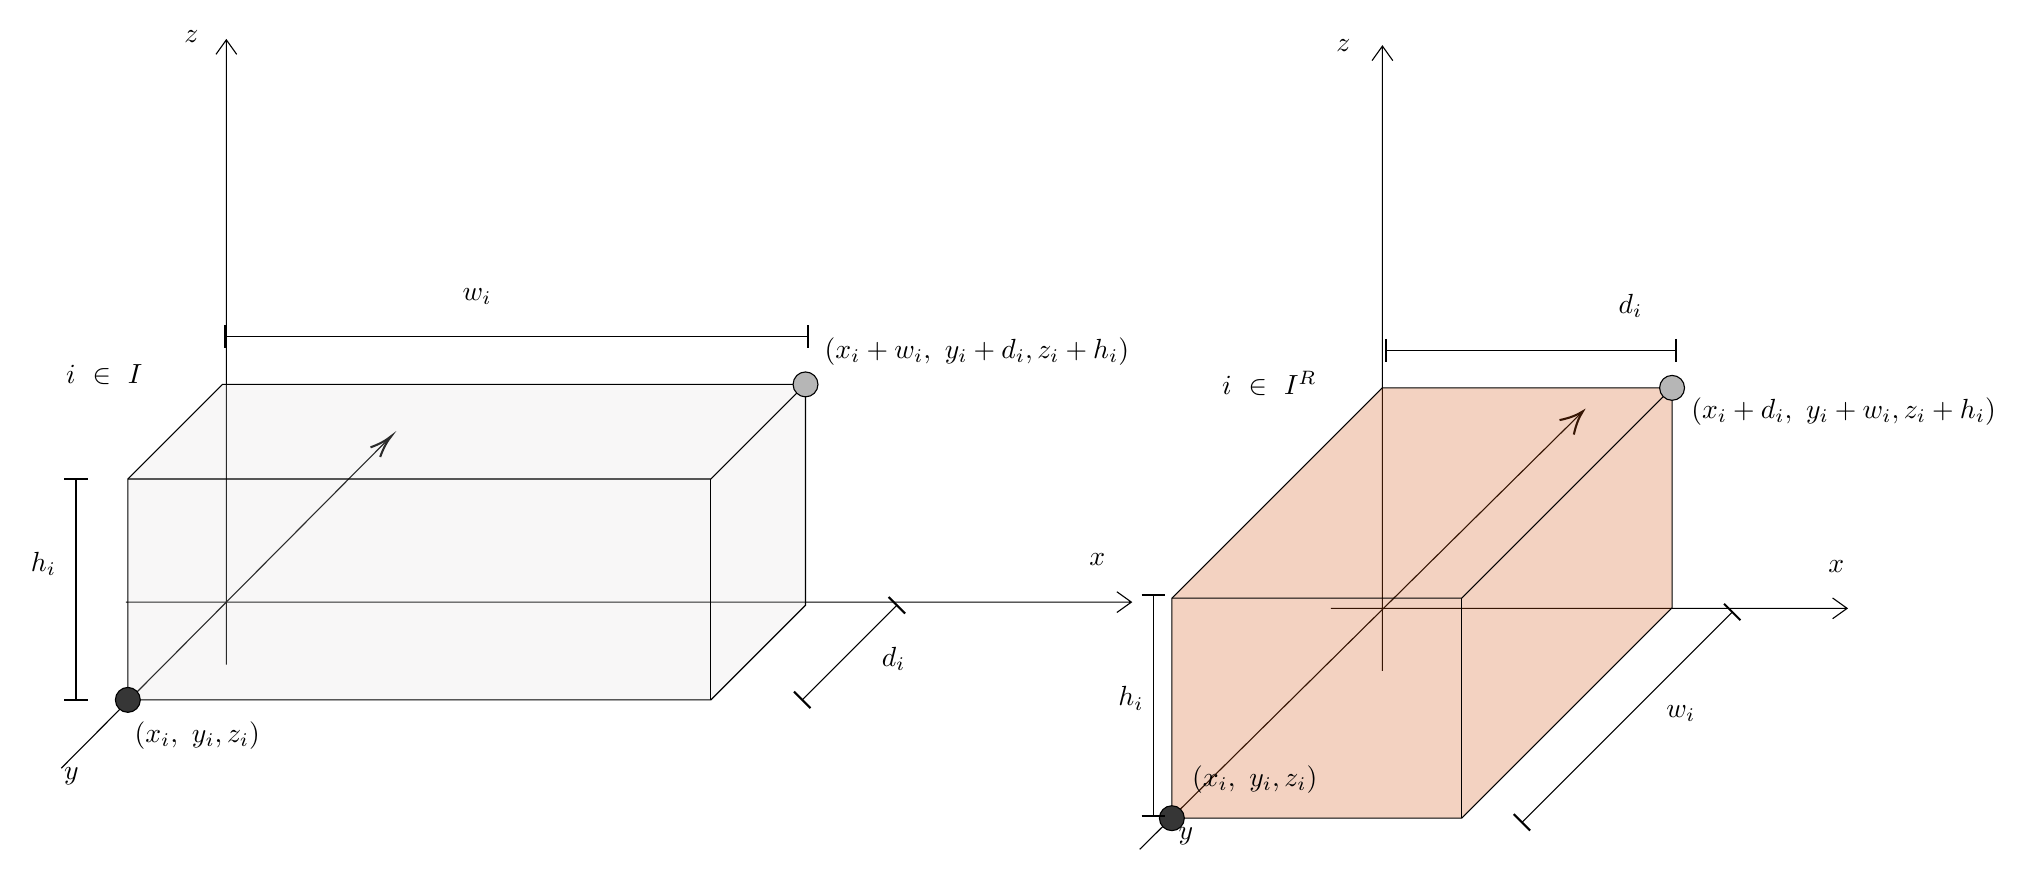
\begin{tikzpicture}[x=0.75pt,y=0.75pt,yscale=-1,xscale=1]
%uncomment if require: \path (0,479); %set diagram left start at 0, and has height of 479

%Shape: Axis 2D [id:dp17090047473688563] 
\draw  (122,295.9) -- (606.5,295.9)(170.45,25) -- (170.45,326) (599.5,290.9) -- (606.5,295.9) -- (599.5,300.9) (165.45,32) -- (170.45,25) -- (175.45,32)  ;
%Straight Lines [id:da9671294084497354] 
\draw    (248.54,217.32) -- (90.95,375.9) ;
\draw [shift={(249.95,215.9)}, rotate = 134.82] [color={rgb, 255:red, 0; green, 0; blue, 0 }  ][line width=0.75]    (10.93,-3.29) .. controls (6.95,-1.4) and (3.31,-0.3) .. (0,0) .. controls (3.31,0.3) and (6.95,1.4) .. (10.93,3.29)   ;
%Shape: Cube [id:dp18105788479145446] 
\draw  [fill={rgb, 255:red, 218; green, 217; blue, 217 }  ,fill opacity=0.2 ] (123,236.6) -- (168.6,191) -- (449.5,191) -- (449.5,297.4) -- (403.9,343) -- (123,343) -- cycle ; \draw   (449.5,191) -- (403.9,236.6) -- (123,236.6) ; \draw   (403.9,236.6) -- (403.9,343) ;
%Flowchart: Connector [id:dp700077731080137] 
\draw  [fill={rgb, 255:red, 54; green, 54; blue, 54 }  ,fill opacity=1 ] (117,343) .. controls (117,339.69) and (119.69,337) .. (123,337) .. controls (126.31,337) and (129,339.69) .. (129,343) .. controls (129,346.31) and (126.31,349) .. (123,349) .. controls (119.69,349) and (117,346.31) .. (117,343) -- cycle ;
%Flowchart: Connector [id:dp7959957780151166] 
\draw  [fill={rgb, 255:red, 182; green, 182; blue, 182 }  ,fill opacity=1 ] (443.5,191) .. controls (443.5,187.69) and (446.19,185) .. (449.5,185) .. controls (452.81,185) and (455.5,187.69) .. (455.5,191) .. controls (455.5,194.31) and (452.81,197) .. (449.5,197) .. controls (446.19,197) and (443.5,194.31) .. (443.5,191) -- cycle ;
%Straight Lines [id:da2736427434795695] 
\draw    (169.6,168) -- (450.5,168) ;
\draw [shift={(450.5,168)}, rotate = 180] [color={rgb, 255:red, 0; green, 0; blue, 0 }  ][line width=0.75]    (0,5.59) -- (0,-5.59)   ;
\draw [shift={(169.6,168)}, rotate = 180] [color={rgb, 255:red, 0; green, 0; blue, 0 }  ][line width=0.75]    (0,5.59) -- (0,-5.59)   ;
%Straight Lines [id:da5491305384137963] 
\draw    (447.9,343) -- (493.5,297.4) ;
\draw [shift={(493.5,297.4)}, rotate = 135] [color={rgb, 255:red, 0; green, 0; blue, 0 }  ][line width=0.75]    (0,5.59) -- (0,-5.59)   ;
\draw [shift={(447.9,343)}, rotate = 135] [color={rgb, 255:red, 0; green, 0; blue, 0 }  ][line width=0.75]    (0,5.59) -- (0,-5.59)   ;
%Straight Lines [id:da2096690092171385] 
\draw    (98,343) -- (98,236.6) ;
\draw [shift={(98,236.6)}, rotate = 90] [color={rgb, 255:red, 0; green, 0; blue, 0 }  ][line width=0.75]    (0,5.59) -- (0,-5.59)   ;
\draw [shift={(98,343)}, rotate = 90] [color={rgb, 255:red, 0; green, 0; blue, 0 }  ][line width=0.75]    (0,5.59) -- (0,-5.59)   ;
%Shape: Axis 2D [id:dp7776925959360946] 
\draw  (702.58,298.9) -- (951.33,298.9)(727.45,28) -- (727.45,329) (944.33,293.9) -- (951.33,298.9) -- (944.33,303.9) (722.45,35) -- (727.45,28) -- (732.45,35)  ;
%Straight Lines [id:da8573442295183169] 
\draw    (822.58,205.41) -- (610.5,415) ;
\draw [shift={(824,204)}, rotate = 135.34] [color={rgb, 255:red, 0; green, 0; blue, 0 }  ][line width=0.75]    (10.93,-4.9) .. controls (6.95,-2.3) and (3.31,-0.67) .. (0,0) .. controls (3.31,0.67) and (6.95,2.3) .. (10.93,4.9)   ;
%Shape: Cube [id:dp7879935806557912] 
\draw  [color={rgb, 255:red, 0; green, 0; blue, 0 }  ,draw opacity=1 ][fill={rgb, 255:red, 209; green, 82; blue, 15 }  ,fill opacity=0.26 ] (626,294) -- (727.33,192.67) -- (867,192.67) -- (867,298.67) -- (765.67,400) -- (626,400) -- cycle ; \draw  [color={rgb, 255:red, 0; green, 0; blue, 0 }  ,draw opacity=1 ] (867,192.67) -- (765.67,294) -- (626,294) ; \draw  [color={rgb, 255:red, 0; green, 0; blue, 0 }  ,draw opacity=1 ] (765.67,294) -- (765.67,400) ;
%Flowchart: Connector [id:dp1932349089965345] 
\draw  [fill={rgb, 255:red, 54; green, 54; blue, 54 }  ,fill opacity=1 ] (620,400) .. controls (620,396.69) and (622.69,394) .. (626,394) .. controls (629.31,394) and (632,396.69) .. (632,400) .. controls (632,403.31) and (629.31,406) .. (626,406) .. controls (622.69,406) and (620,403.31) .. (620,400) -- cycle ;
%Flowchart: Connector [id:dp6515973139480861] 
\draw  [fill={rgb, 255:red, 182; green, 182; blue, 182 }  ,fill opacity=1 ] (861,192.67) .. controls (861,189.36) and (863.69,186.67) .. (867,186.67) .. controls (870.31,186.67) and (873,189.36) .. (873,192.67) .. controls (873,195.99) and (870.31,198.67) .. (867,198.67) .. controls (863.69,198.67) and (861,195.99) .. (861,192.67) -- cycle ;
%Straight Lines [id:da6236125294574628] 
\draw    (729.33,174.67) -- (869,174.67) ;
\draw [shift={(869,174.67)}, rotate = 180] [color={rgb, 255:red, 0; green, 0; blue, 0 }  ][line width=0.75]    (0,5.59) -- (0,-5.59)   ;
\draw [shift={(729.33,174.67)}, rotate = 180] [color={rgb, 255:red, 0; green, 0; blue, 0 }  ][line width=0.75]    (0,5.59) -- (0,-5.59)   ;
%Straight Lines [id:da29019630748971836] 
\draw    (794.67,402) -- (896,300.67) ;
\draw [shift={(896,300.67)}, rotate = 135] [color={rgb, 255:red, 0; green, 0; blue, 0 }  ][line width=0.75]    (0,5.59) -- (0,-5.59)   ;
\draw [shift={(794.67,402)}, rotate = 135] [color={rgb, 255:red, 0; green, 0; blue, 0 }  ][line width=0.75]    (0,5.59) -- (0,-5.59)   ;
%Straight Lines [id:da5655913131564809] 
\draw    (617,399) -- (617,292.6) ;
\draw [shift={(617,292.6)}, rotate = 90] [color={rgb, 255:red, 0; green, 0; blue, 0 }  ][line width=0.75]    (0,5.59) -- (0,-5.59)   ;
\draw [shift={(617,399)}, rotate = 90] [color={rgb, 255:red, 0; green, 0; blue, 0 }  ][line width=0.75]    (0,5.59) -- (0,-5.59)   ;

% Text Node
\draw (125,352.4) node [anchor=north west][inner sep=0.75pt]    {$( x_{i} ,\ y_{i} ,z_{i})$};
% Text Node
\draw (457.45,167.3) node [anchor=north west][inner sep=0.75pt]    {$\left( x_{i} + w_{i} ,\ y_{i} + d_{i} ,z_{i} +h_{i}\right)$};
% Text Node
\draw (92,180.4) node [anchor=north west][inner sep=0.75pt]    {$i \ \in\ I$};
% Text Node
\draw (283,143.4) node [anchor=north west][inner sep=0.75pt]    {$w_{i}$};
% Text Node
\draw (485,316.4) node [anchor=north west][inner sep=0.75pt]    {$d_{i}$};
% Text Node
\draw (75,270.4) node [anchor=north west][inner sep=0.75pt]    {$h_{i}$};
% Text Node
\draw (634.45,373.3) node [anchor=north west][inner sep=0.75pt]    {$( x_{i} ,\ y_{i} ,z_{i})$};
% Text Node
\draw (875,196.07) node [anchor=north west][inner sep=0.75pt]    {$\left( x_{i} + d_{i} ,\ y_{i} + w_{i} ,z_{i} +h_{i}\right)$};
% Text Node
\draw (649,183.4) node [anchor=north west][inner sep=0.75pt]    {$i \ \in\ I^R$};
% Text Node
\draw (840,146.4) node [anchor=north west][inner sep=0.75pt]    {$d_{i}$};
% Text Node
\draw (863,344.4) node [anchor=north west][inner sep=0.75pt]    {$w_{i}$};
% Text Node
\draw (599,335.4) node [anchor=north west][inner sep=0.75pt]    {$h_{i}$};
% Text Node
\draw (149,19.4) node [anchor=north west][inner sep=0.75pt]    {$z$};
% Text Node
\draw (704,23.4) node [anchor=north west][inner sep=0.75pt]    {$z$};
% Text Node
\draw (941,274.4) node [anchor=north west][inner sep=0.75pt]    {$x$};
% Text Node
\draw (585,271.4) node [anchor=north west][inner sep=0.75pt]    {$x$};
% Text Node
\draw (91,374.4) node [anchor=north west][inner sep=0.75pt]    {$y$};
% Text Node
\draw (628,403.4) node [anchor=north west][inner sep=0.75pt]    {$y$};


\end{tikzpicture}

    }
    \caption{Coordinate system representation for a generic item $i$ and it's rotated clone $i \in I^R$}
    \label{fig:coordinate_system}
\end{figure}

The 3D-SBSBPP can then be formulated as a mixed-integer linear programming problem:
\label{par:standard_const}
\begin{align}
   \min       \qquad& \sum\limits_{b \in B} (H v_b + z^{max}_b) & \label{eq:objective} \\
   \text{s.t.} \qquad& \sum\limits_{b \in B}{u_{ib}} = 1 & \forall i \in I  \label{cons:all_items_in_bin} \\
                    & u_{ib} \le v_b & \forall i \in I, \forall b \in B \label{cons:items_in_used_bins} \\
                    & v_b \ge v_c & \forall (b,c) \in B : b < c  \label{cons:bin_breaking} \\
                    & x_i + w_i \le W & \forall i \in I \label{cons:inside_x} \\ 
                    & y_i + d_i \le D & \forall i \in I \label{cons:inside_y} \\ 
                    & z_i + h_i \le H & \forall i \in I \label{cons:inside_z} \\ 
                    & z^{max}_b \ge (z_i + h_i) - H(1-u_{ib}) & \forall i \in I, \forall b \in B \label{cons:maxz} \\
                    & (x_i + w_i) - x_j\le W(1 - x^p_{ij}) & \forall i,j \in I \label{cons:x_prec_1} \\
                    & x_j - (x_i + w_i) + 1 \le W x^p_{ij} & \forall i,j \in I \label{cons:x_prec_2} \\
                    & (y_i + d_i) - y_j \le D(1 - y^p_{ij}) & \forall i,j \in I \label{cons:y_prec_1} \\
                    & y_j - (y_i + d_i) + 1 \le D y^p_{ij} & \forall i,j \in I \label{cons:y_prec_2} \\
                    & (z_i + h_i) - z_j\le H(1 - z^p_{ij}) & \forall i,j \in I \label{cons:z_prec_1} \\
                    & z_j - (z_i + h_i) + 1 \le H z^p_{ij} & \forall i,j \in I \label{cons:z_prec_2} \\
                    & x^p_{ij} + x^p_{ji} + y^p_{ij} + y^p_{ji} + z^p_{ij} + z^p_{ji} \ge u_{ib} + u_{jb} - 1 & \forall i,j \in I, \forall b \in B \label{cons:no_overlap}
\end{align}

The objective function \ref{eq:objective} seeks to minimize the number of opened bins and the maximum heights of the opened bins.
In a single bin configuration since all the volume mass is concentrated inside one bin this also means that it maximises the cage ratio.
Constraint \ref{cons:all_items_in_bin} ensures that each item is packed in one and only one bin, while contraint \ref{cons:items_in_used_bins} ensures that items are only packed in bins that are used in the solution.
Since the solution as lots of simmetries with respects to the number of bins a simmetry breaking constraint \ref{cons:bin_breaking} can be added on the opening of bins to improve solve times.
Each item is also ensured to be placed inside the bin thanks to \cref{cons:inside_x,cons:inside_y,cons:inside_z}.
The value of $z^{max}_b$ is forced to converge to the maximum height of a given bin thanks to constraint \ref{cons:maxz}.
Constraints from \ref{cons:x_prec_1} to \ref{cons:z_prec_2} are used to define the precedence binary variables $x^p_{ij}$, $y^p_{ij}$, $z^p_{ij}$ over each axis as described in the problem formulation.
Constraint \ref{cons:no_overlap} then ensures that if two items are in the same bin then there needs to be at least one axis with a clear order of precedence, otherwise the two items would be overlapping eachother.
\subsection{Othogonal rotations}
\label{subsec:orthogonal_rotations}%

Let us extend the definition of the bin packing problem without rotations with a new formulation which allows $90$ degrees rotations of each item.
Let $I = I^O \cup I^R$ be the new set of items where $I^O$ is the set of original non-rotated items and $I^R$ is the set of items rotated by $90$ degrees.
Given the set of tuples $(i, j) \in I^{OR}$ where $i$ is the original item with dimensions $(w_i, d_i, h_i)$ and $j$ is the corresponding rotated clone with dimensions $(w_j, d_j, h_j) = (d_i, w_i, h_i)$, we can now rewrite constraint \ref{cons:all_items_in_bin} as \ref{cons:all_items_in_bin_with_rotation} to force only one for the item between the original and rotated to be part of the solution.

\begin{align}
    & \sum\limits_{b \in B} u_{ib} + \sum\limits_{b \in B} u_{jb} = 1 & \forall (i, j) \in I^{OR} \label{cons:all_items_in_bin_with_rotation}
\end{align}

\subsection{Discrete vertical support formulation}
\label{subsec:vertical_support_formulation}%

We now extend the model to address the constraint of static support. 
In the literature there are some mathematical formulations that tackle the concept of area support, and in some cases vertex support. In \citeauthor{elhedhli2019three} a SOCP formulation of the support constraint was used but was limited to the problem of spacing between layers with one of the layers being fixed in position, in our case a similar formulation would lead to a non-linear support constraint.
By introducing a discretization over the XY-plane a linear version of the constraint can be formulated similar to the one proposed in \citeauthor{kurpel2020exact} without the need to discretize the z-axis as well.

Let us introduce some additional parameters to the model, let $0 \le \alpha_s \le 1$ be the ammount of area that an item needs to have supported by other items and let $\beta_s$ be the height tollerance to consider one item as being close enough to support another item (as seen in \cref{fig:support}).
In addition to the support parameters an additional parameter $\delta$ is given which rappresents the discretization unit used to partition the XY-plane. Let $I^B$ be the set of all the tuples $(i, j, b)$ such that $(i,j) \in I \land i \neq j$ and $b \in B$.
We can now compute a few additional parameters that will be used to reduce the number of constraints evaluated by the model. Let $\gamma$ be the maximum size over a dimension on the XY-plane between all the items as \cref{eq:gamma_max_dim}, and let $\Delta$ be the set of all possible distances between the origins of two items along one discretized axis as \cref{eq:Delta_possible_diffs}.
\begin{align}
    \gamma = \max_{\forall i \in I}\{ w_i, d_i \} \label{eq:gamma_max_dim} \\
    \Delta =  \left[ - \left\lfloor \frac{ \gamma }{\delta} \right\rfloor, \left\lfloor \frac{ \gamma }{\delta} \right\rfloor \right] \label{eq:Delta_possible_diffs}
\end{align}
Let $O(i, j, h, k) \rightarrow \mathbb{R}^+$ be a function that computes the ammount of overlap between two items $(i,j) \in I$ given the discretized distance between each other $(h, k) \in \Delta$ such that $x_j = x_i + \delta h$ and $y_j = y_i + \delta k$ which returns the area of overlap or 0 otherwhise.

Additional new variables need to be added to the ones of the original model, let $s_{ij}$ be a set of binary variables which will assume value 1 if item $i \in I$ can offer support to item $j \in I$ and 0 otherwhise. A new set of binary variables $z^c_{ij}$ will be 1 if item $i \in I$ is close w.r.t. the z-axis to item $j \in I$, which would mean that $z_j - (z_i + h_i) \le \beta_s$, and 0 otherwhise.
Let us then introduce a new set of binary variables $g_i$ which will assume value 1 if item $i \in I$ will be on the ground or 0 otherwhise and a set of binary variables $s^{kh}_{i j b}$ that will assume value 1 if item $i \in I$ will receive support from item $j \in I$ and both will be placed in bin $b \in B$ with a discretized distance of $(k, h) \in \Delta$ between eachother and 0 otherwise.

Given all the additional parameters and variables introduced, a new formulation of the model can be given with the same objective function \ref{eq:objective} and the constraints in \cref{par:standard_const} with the addition of the following constraints:
\label{par:support_const}
\begin{align}
    & z_j - (z_i + h_i) \le \beta_s + H (1 - z^c_{ij}) & \forall (i, j) \in I : i \neq j \label{cons:z_close_1} \\
    & z_j - (z_i + h_i) \ge -\beta_s - H (1 - z^c_{ij}) & \forall (i, j) \in I : i \neq j \label{cons:z_close_2} \\
    & s_{ij} \le z^p_{ij} & \forall (i, j) \in I  \label{cons:supporting_1} \\
    & s_{ij} \le z^c_{ij} & \forall (i, j) \in I  \label{cons:supporting_2} \\
    & s_{ij} \ge z^p_{ij} + z^c_{ij} - 2 & \forall (i, j) \in I : i \neq j \label{cons:supporting} \\
    & \sum\limits_{j \in I}{s_{ij}} \le \sum\limits_{b \in B}{u_{ib}} & \forall i \in I  \label{cons:support_comes_from_placed} \\
    & z_i \le H(1 - g_i) & \forall i \in I \label{cons:grounded} \\
    & \sum\limits_{(k, h) \in \Delta, b \in B : O(i, j, k, h) \neq 0} s^{k h}_{i j b} \le s_{ij} & \forall (i, j) \in I \label{cons:discretized_support_same} \\
    & \sum\limits_{(k, h) \in \Delta : O(i, j, k, h) \neq 0} s^{k h}_{i j b} \le u_{ib} & \forall (i, j, b) \in IB \label{cons:discretized_support_right_bin_i} \\
    & \sum\limits_{(k, h) \in \Delta : O(i, j, k, h) \neq 0} s^{k h}_{i j b} \le u_{jb} & \forall (i, j, b) \in IB \label{cons:discretized_support_right_bin_j}
\end{align}
Constraints \ref{cons:z_close_1} and \ref{cons:z_close_2} ensure that $z^c_{ij}$ is forced to 1 only when the distance over the z-axis between item $i$ and item $j$ is within the range $[-\beta_s, \beta_s]$.
The value of $s_{ij}$ is then assigned to the logical equation $z^p_{ij} \land z^c_{ij}$ thanks to constraints from \ref{cons:supporting_1} to \ref{cons:supporting}.
Since some items could be left out of the solution due to the formulation of orthogonal rotations, we also ensure that support can only come from placed items thanks to constraint \ref{cons:support_comes_from_placed}.
Constraint \ref{cons:grounded} together with the hard constraint of support that will be introduced ensures that the $g_i$ assumes value 1 if item $i$ is on the ground.
Constraints from \ref{cons:discretized_support_same} to \ref{cons:discretized_support_right_bin_j} ensure that if a discretized support decision $s_{ijb}^{hk}$ is 1 then every subscript of that variable must be true in the non-discretized model, so item $i$ can give discretized support to item $j$ in in bin $b$ if both items are are assinged to bin $b$ and if $i$ can give support to item $j$. They also force the selection of only one possible combination of $(h,k) \in \Delta$ for which $i$ gives support to $j$.

We can then define a set of constraints which given a discretized placement $s^{k h}_{i j b}$ limits the distance between $i$ and $j$ to a given continuous region in space delimited by a square of the dimmension of our discretization unit $\delta$. 
Given every tuple of possible discretized distances between items $ (k, h) \in \Delta$ and every tuple of different pairs of items in the same bin $(i, j, b) \in I^B$ such that the items would overlap over the discretized plane XY for a non-null region ($O(i, j, k, h) \neq 0$) the resulting constraints are defined in \cref{cons:discretized_support_limit_x_1,cons:discretized_support_limit_x_2,cons:discretized_support_limit_y_1,cons:discretized_support_limit_y_2}.
\begin{align}
    & x_j - x_i \ge \gamma k - 2W( 1 - s^{k h}_{i j b}) &  \label{cons:discretized_support_limit_x_1} \\
    & x_j - x_i \le \gamma (k + 1) + 2W( 1 - s^{k h}_{i j b}) &  \label{cons:discretized_support_limit_x_2} \\
    & y_j - y_i \ge \gamma h - 2D( 1 - s^{k h}_{i j b}) &  \label{cons:discretized_support_limit_y_1} \\
    & y_j - y_i \le \gamma (h + 1) + 2D( 1 - s^{k h}_{i j b}) &  \label{cons:discretized_support_limit_y_2}
\end{align}

And finally we can introduce a feasibility constraint which ensures that every item that isn't on the ground is supported by other items placed beneath it by at least $\alpha_s$ times its area, which corresponds to condition \ref{support:area_support} of the pratical constraint of vertical support.
\begin{eqnarray}
    & \sum\limits_{(k, h) \in \Delta, b \in B, j \in I : i \neq j \land O(i, j, k, h) \neq 0}{ O(i, j, k, h)s^{k h}_{j i b}} \ge \alpha_s w_i d_i - w_i d_i g_i & \forall i \in I \label{cons:every_item_is_supported}
\end{eqnarray}